\documentclass{article}
\usepackage{setspace}
\usepackage{amsfonts}
\usepackage{graphicx}
\usepackage{amsmath}
\graphicspath{{./figures/}}
 
%----------------------------------------------------------------------------------------
%     AUTHORS and ABSTRACT
%----------------------------------------------------------------------------------------

\title{Initializing Molecular Dynamics with Low Discrepancy Sequences}
\author{Jacob Price, Gil Shohet, Michael S. Murillo}

\begin{document}
\maketitle

\begin{abstract}
Molecular dynamics simulations are often initialized without regard for interparticle correlations. This frequently results in an inadvertent excess of potential energy that is converted to kinetic energy in the initial steps of simulation, resulting in an increase in temperature. To counteract this, a long equilibration phase with a thermostat algorithm precedes the actual simulation. We propose here a new method for minimizing the length of the equilibration phase by initializing ions using low-discrepancy sequences that distribute initial positions nearly uniformly throughout the domain. These initial positions can be precomputed deterministically, and can be used to minimize the computational time and effort that must be dedicated to driving an initial distribution toward the desired ensemble, lowering the computational burden for molecular dynamics simulations.
\end{abstract}

\pagebreak

%----------------------------------------------------------------------------------------
\section{Introduction}
%----------------------------------------------------------------------------------------

Since its inception \cite{fermi1955studies}, molecular dynamics (MD) simulations have been a versatile tool for investigating microscopic details in chemical, physical, and biological systems. By tracking molecular trajectories, systems are understood at a greater level of detail than when they are treated with a continuum model.

In an MD simulation, an $N$-body system is numerically solved yielding dynamical trajectories of individual atoms, ions, or molecules in the system. These trajectories can be used to compute observable quantities as ensemble averages of dynamical states. Examples include transport coefficients, fluxes, stress tensors, and thermodynamic properties such as pressure and temperature. MD simulations are also useful for sampling statistical mechanical ensembles to determine equilibrium and nonequilibrium properties. For an overview of molecular dynamics simulations, see \cite{tuckerman2000understanding}.

The interparticle potential functions govern the explicit motion of particles and determine their interactions. By altering the interparticle potential, a variety of physical, chemical, and biological phenomena can be explored with minimal changes to simulation algorithms. With a Coulomb potential, MD can simulate classical electrodynamic motion. The Yukawa potential approximates electron screening in neutral plasma simulations. The Lennard-Jones potential models neutral atom motion. The hard sphere potential allows for the study of neutral spheres undergoing elastic collisions. These are only some of the many interparticle potentials that can be employed, and their variety demonstrate the flexibility and utility of MD simulations.

%\begin{equation}
%\begin{split}
%\frac{\partial \mathbf{r}_i}{\partial t}&=\frac{1}{m_i}\nabla_{\mathbf{v}_i} H\\
%\frac{\partial \mathbf{v}_i}{\partial t}&=-\frac{1}{m_i}\nabla_{\mathbf{r}_i}H\\
%H(\{\mathbf{r}_k\}_{k=1}^N,\{\mathbf{v}_k\}_{k=1}^N)&=\sum_\alpha\left[\frac{m_\alpha|\mathbf{v}_\alpha|^2}{2}+\sum_{\alpha<j}U_{\alpha j}(\mathbf{r}_\alpha,\mathbf{r}_j)\right],
%\end{split}
%\label{eq:hamiltonian}
%\end{equation}

There are two distinct classes of MD simulations: equilibrium molecular dynamics (EMD) and nonequilibrium molecular dynamics (NEMD). In both cases, the temperature of the system is a critical parameter. In EMD, we are interested in the equilibrium properties of a system subject to thermodynamic constraints. The most common is the microcanonical ensemble, which has fixed energy, volume, and particle count. In NEMD, we are interested in dynamical properties such as absorption spectra and rate constants.

In both cases, we are interested observing the evolution of a system whose initial state is prescribed by the researcher in terms of macroscopic observables. When simulating an equilibrium state, we wish to specify the temperature, volume, and particle count. When simulating nonequilibrium dynamics, we wish to initialize the system in a state consistent with the desired thermodynamic properties of the initial state. While the volume and particle count are easy to initialize with the proper values, the temperature proves more difficult.

The temperature of an MD simulation is defined to be proportional to the total kinetic energy of the system. Theoretically, we can initialize a distribution with a well-defined temperature by sampling velocities for our particles from a velocity distribution with the desired variance, frequently a Maxwellian. In practice, however, this is only part of the story. The desired temperature provides a distribution from which to sample velocities, but it is unclear how to select the initial positions of particles. A natural strategy is to select positions from a uniform distribution. This does not, however, take into account particle correlations that would be present in a physical system. Two particles might be randomly placed much closer together than would typically occur given their interparticle potential. As an extreme case, if we are modeling solid spheres and we place them randomly, we might place them such that the spheres would be overlapping --- a physical impossibility.

The consequence of this uncertainty is that random placement of particles results in a higher potential energy than would be observed in reality. When Hamiltonian dynamics are evolved with a symplectic integrator, such as the Verlet algorithm \cite{verlet1967computer}, MD simulations conserve total energy. This is one of the most attractive features of MD, but it also causes some difficulties in initializing physically relevant simulations. We often wish to simulate the microcanonical ensemble, but with a well-defined initial temperature. However, once the simulation begins, the particles move to find a minimum potential energy. The excess potential energy that was inadvertently added to the system is converted into kinetic energy, and the temperature increases. A real world example of this ``disorder induced heating'' is described in \cite{gericke2003disorder}.

There are a number of solutions to the problem of disorder induced heating. First, thermostat algorithms, such as velocity scaling, the Nos\'e-Hoover chain, or Langevin dynamics can be used to simulate connecting the system to a constant temperature heat bath. Once the initial distribution results in a temperature spike, excess kinetic energy is drained from the system into the bath, equilibrating the system temperature to the prescribed temperature as the particles move to a minimum potential energy distribution. Depending on the target temperature and the size of the initial energy spike, this method can take up considerable computational time. Another solution is the radius rejection algorithm. In this, positions are drawn from a uniform distribution, then compared against the previously placed particles. If the proposed particle is at least $r_0$ away from all other particles, it is kept. Otherwise, it is rejected. This method is computationally intensive, especially as the number of particles is increased. Furthermore, it requires an ad hoc choice of the minimum distance $r_0$.  The system will still require an equilibration phase, but ideally there will be a smaller temperature spike, and the thermostat will have to spend less time adjusting the energy to the proper level.

In this paper, we provide a brief overview of MD simulation. We then introduce discrepancy as a means of formalizing the logic behind the radius rejection initialization method described above. We introduce low-discrepancy sequences, which provide a deterministic alternative for selecting initial positions with desirable properties. Finally, we propose a new scheme capitalizing on these sequences to minimize the computational cost of initializing an MD simulation with a target temperature.

%----------------------------------------------------------------------------------------
\section{Molecular Dynamics Simulation}
%----------------------------------------------------------------------------------------

Consider a system of $N$ particles with positions $\mathbf{x}_1,\dots,\mathbf{x}_N$ and velocities $\mathbf{v}_1,\dots,\mathbf{v}_N$. Molecular dynamics simulations numerically solve Newton's equations of motion for this many-body system:
\begin{equation}
m_i \ddot{\mathbf{x}}_i=\mathbf{F}_i
\end{equation}where $\mathbf{F}_i$ is the force on particle $i$. In general, the problem is often reformulated in terms of Hamiltonian dynamics. Let the Hamiltonian of the system be
\begin{equation}
H(\mathbf{x}_1,\dots,\mathbf{x}_N,\mathbf{v}_1,\dots,\mathbf{v}_N)=\sum_{i=1}^N \frac{m_i \mathbf{v}_i^2}{2}+U(\mathbf{r}_1,\dots,\mathbf{r}_N),
\end{equation}where $U$ is the interparticle potential such that
\begin{equation}
\mathbf{F}_i=-\frac{1}{m_i}\frac{\partial U}{\partial \mathbf{r}_i}.
\end{equation}

Then, the Hamiltonian equations of motion are
\begin{align}
\begin{split}
\dot{\mathbf{r}}_i=&\frac{1}{m_i}\frac{\partial H}{\partial \mathbf{v}_i}=\mathbf{v}_i\\
\dot{\mathbf{v}}_i=-\frac{1}{m_i}\frac{\partial H}{\partial \mathbf{x}_i}=-&\frac{1}{m_i}\frac{\partial U}{\partial \mathbf{x}_i}=\mathbf{F}_i(\mathbf{x}_1,\dots,\mathbf{x}_N).
\end{split}\label{hamiltonian}
\end{align}

Coupled with an initial condition $\mathbf{x}_1(0),\dots,\mathbf{x}_N(0),\mathbf{v}_1(0),\dots,\mathbf{v}_N(0)$, this forms a set of $N$ ordinary differential equations uniquely defining the trajectory of the initial condition. They can be numerically integrated to generate a simulated trajectory.

Hamiltonian dynamics conserve energy, and it is desirable for this to be reflected in the numerical solution. Consequently, symplectic integrators are typically used to numerically solve this system. A classic example is the velocity Verlet algorithm, a second order scheme. Let $\Delta t$ be the size of the time step. Then the scheme is:
\begin{equation}
\begin{split}
\mathbf{v}_i\left(t+\frac{\Delta t}{2}\right)  	&= \mathbf{v}_i(t) + \frac{\Delta t}{2}\frac{\mathbf{F}_i(t)}{m_i} \\
\mathbf{r}_i(t+\Delta t) 		   		&= \mathbf{r}_i(t) + \Delta t\:\mathbf{v}_i\left(t+\frac{\Delta t}{2}\right) \\
\mathbf{v}_i(t+\Delta t)			  	&= \mathbf{v}_i\left(t+\frac{\Delta t}{2}\right) + 
								\frac{\Delta t}{2}\frac{\mathbf{F}_i(t+\Delta t)}{m_i}.
\end{split}\label{verlet}
\end{equation}

It is typically not the case that the explicit initial condition is known. Instead, we often desire an initial condition consistent with macroscopic observables, such as temperature and pressure. These states, however, are not known \emph{a priori}. Therefore, we select a guess for the initial condition, and during an equilibration phase drive the system in some way toward a state with the desired macroscopic quantities.

Most frequently, the desired macroscopic quantity is the system temperature. The instantaneous temperature of an MD system is defined as
\begin{equation}
T(\mathbf{v}_1,\dots,\mathbf{v}_N)=\frac{2k_B}{3N}\sum_{i=1}^N\frac{m_i\mathbf{v}_i^2}{2}.
\end{equation}The dynamics must be altered in order to drive the system toward a desirable temperature. There are a number of techniques to accomplish this, and all employ a dynamical ``equilibration phase'' that precedes the true initial state of the simulation.

In the velocity scaling method, during the equilibration phase the observed velocities are uniformly rescaled such that the temperature of the system matches the desired temperature.

In the Nos\'e-Hoover and Langevin dynamical methods, the equations of motion are altered to simulate coupling the system to a heat bath of the desired temperature. For example, in Langevin dynamics, the Hamiltonian equations (\ref{hamiltonian}) are modified to
\begin{equation}
\begin{split}
\dot{\mathbf{r}}_i=&\mathbf{v}_i\\
\dot{\mathbf{v}}_i=\mathbf{F}_i(\mathbf{x}_1,\dots,\mathbf{x}_N)-&\gamma_i \mathbf{v}_i+\sqrt{2\gamma_i k_BTm_i}R(t)
\end{split}\label{langevin}
\end{equation}where $\gamma_i$ is the a parameter representing the degree to which particle $i$ is coupled to the heat bath, $T$ is the desired system temperature, and $R(t)$ is a delta-correlated stationary zero-mean Gaussian process. The resulting integration scheme is
\begin{align}
\mathbf{v}_i\left(t+\frac{\Delta t}{2}\right) &= \mathbf{v}_i(t) + \frac{\Delta t}{2}\frac{\mathbf{F}_i(t)}{m_i} - \frac{\gamma_i\Delta t}{2}\mathbf{v}_i(t) + \sqrt{\frac{\gamma_i \Delta tT}{m_i}}\eta_1 \notag\\
\mathbf{r}_i(t+\Delta t) &= \mathbf{r}_i(t) + \Delta t\mathbf{v}_i\left(t+\frac{1}{2}\Delta t\right) \label{langevinverlet}\\
\mathbf{v}_i(t+\Delta t) &= \left(1 + \frac{\gamma_i\Delta t}{2}\right)^{-1} \left(\mathbf{v}_i\left(t+\frac{\Delta t}{2}\right) +  \frac{\Delta t}{2}\frac{\mathbf{F}_i(t+\Delta t)}{m_i} + \sqrt{\frac{\gamma_i \Delta tT}{m_i}}\eta_2\right).\notag
\end{align}where $\eta_1$ and $\eta_2$ are independent samples of the standard Gaussian distribution. Evolving any initial condition according to these dynamics will drive it toward a distribution with the desired temperature by draining energy from the system via the frictional term $\gamma_i\mathbf{v}_i$. The rate of convergence can be adjusted by selecting different values for the coupling parameter $\gamma_i$.

It is only after this equilibration phase is complete that the distribution is considered the ``true'' initial condition and the actual simulation can begin. The following sections will demonstrate the profound role played by the initial guess prior to the equilibration phase.

%----------------------------------------------------------------------------------------
\section{Low-Discrepancy Sequences}
%----------------------------------------------------------------------------------------

Consider $N$ points $\mathbf{x}_1,\dots,\mathbf{x}_N$ in the $s$-dimensional unit cube $I_s$. Let $A$ be some sub-interval of $I_s$ with volume $V(A)$. Define $P(A)$ as the proportion of points in $\{\mathbf{x}_i\}_{i=1}^N$ that fall in the sub-interval $A$. Then the discrepancy $D$ of the sequence $\{\mathbf{x}_i\}_{i=1}^N$ is defined as
\begin{equation}
D\left(\{\mathbf{x}_i\}_{i=1}^N\right)=\sup_A\left[P(A)-V(A)\right].
\end{equation}In a sense, a set of points with a low discrepancy covers the unit cube such that the proportion of points in any volume $A$ is approximately equal to the volume of $A$. Low-discrepancy sequences can be constructed that satisfy
\begin{equation}
D\left(\{\mathbf{x}_i\}_{i=1}^N\right)\leq B_s(\log N)^{s-1}+O((\log N)^{s-2})
\end{equation}and 
\begin{equation}
D\left(\{\mathbf{x}_i\}_{i=1}^N\right)\leq C_s(\log N)^{s}+O((\log N)^{s-1})
\end{equation}for constants $B_s$ and $C_s$. Figure \ref{fig:halton} demonstrates the difference between a random sampling on the unit square and a low-discrepancy sequence in terms of uniformity of points. Deterministic sequences that aim to minimize $B_s$ and $C_s$, called quasi-random sequences, have been constructed \cite{niederreiter1988low}. In order of decreasing $B_s$ and $C_s$, these sequences are those constructed by Halton \cite{halton1960efficiency}, Sobol' \cite{soboldistribution}, Faure \cite{faure1982discrepance}, and Neiderreiter \cite{niederreiter1987point}.

\begin{figure}
\center 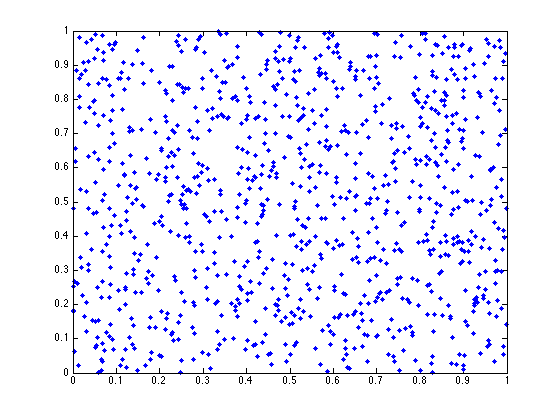
\includegraphics[width=0.8\linewidth]{random.png}\\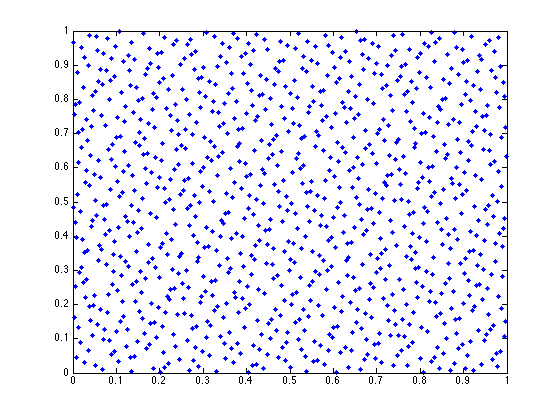
\includegraphics[width=0.8\linewidth]{halton.png}
\caption{(Top) $N=1000$ points selected from a uniform distribution on the unit square. (Bottom) $N=1000$ points selected using the Halton sequence with base two for the $x$-coordinate and the Halton sequence with base three for the $y$-coordinate. Note the roughly uniform covering of the unit square in the lower image, with minimal clustering of points compared against the top image.}
\label{fig:halton}
\end{figure}

It is important to note that  quasi-random sequences are deterministic and have relatively simple algorithms \cite{dalal2008low}. They can be precomputed and then used repeatedly. Variations with the same low discrepancy can be constructed by permuting the indices of each coordinate (``scrambling'') \cite{mascagni2004scrambled}. Furthermore, the addition of new points does not require comparisons against old points, as in the radius rejection method. The computational cost of generating quasi-random sequences is negligible, as they need only be computed once. Quasi-random sequences have been used in optics \cite{ide2003dot}, mathematical finance \cite{ninomiya1996toward}, and Monte Carlo integration methods \cite{dalal2008low,halton1960efficiency,mascagni2004scrambled,morokoff1994quasi,soboldistribution} with great results. 

We will now demonstrate that intelligently selected quasi-random sequences can also drastically decrease the amount of temperature increase in the initial steps of an MD simulation, and thus decrease the computational cost of driving the system to the desired temperature with a thermostat.

\section{Analysis}

In MD, the radial distribution function $g(r)$ is used to quantify the degree of correlation of simulated particles, normalized against the fully uncorrelated ideal gas case. For a collection of $N$ particles at positions $\mathbf{x}_1,\dots,\mathbf{x}_N$, $g(r)$ is defined as:
\begin{equation}
g(r)\,dr=\frac{d(r) V}{4\pi r^2 N}
\end{equation}where $d(r)$ is the observed number of interparticle distances $|\mathbf{x}_i-\mathbf{x}_j|$, $i\neq j$, between $r$ and $r+dr$. This quantity can be approximated by creating a histogram of interparticle distances. Figure \ref{fig:radialdist} depicts examples of radial distribution functions for randomly placed points as well as points placed with various low-discrepancy sequences.

\begin{figure}
\caption{Radial distribution functions computed for a random selection of $N=1000$ points and for various low-discrepancy sequences of $N=1000$ points.}
\label{fig:radialdist}
\end{figure}

Any given interparticle potential $U$ and desired temperature $T$ has a unique radial distribution function $g(r)$ associated with it. In a sense, the initialization problem is to select a distribution of particles with this desired $g(r)$. If this desired distribution function is known, the nearer to this desired shape our initial distribution is, the less time will need to be spent driving it to the proper correlations.

Here, for several commonly used interparticle potentials, we demonstrate how to select the initial distribution whose radial distribution function best approximates the projected radial distribution function given a specific temperature.

\section{Conclusion}

We have demonstrated the benefits of selecting a low-discrepancy sequence for initializing the positions of particles in a molecular dynamics simulation. First, the sequences are deterministic, and thus can be precomputed or included in an MD package and used for essentially no computational cost. This is an advantage over the radius rejection method, which requires every additional point be compared against every prior point, and initializing more points takes more and more computational time. Second, the sequences and parameters can be selected in such a way that their radial distribution functions roughly approximate the target initial radial distribution function. This reduces the length of time that must be spent in the equilibration phase.

We can capitalize upon these advantages best by implementing these sequences directly into an MD package. A desired potential, initial temperature, and number of particles can be specified by the user, and the package will automatically select a set of points that will reach that initialization very quickly.

The benefits of this method increase as the number of particles in a simulation increase. The equilibration phase involves particle evolution, so the amount of computational time spent there increases like $O(N)$ or worse. This computational time is particularly undesirable since it occurs prior to the actual relevant simulation. Low discrepancy sequences offer a means to minimize the preparation steps before an MD simulation. As MD simulations grow to millions or billions of particles, this new approach will prove invaluable.

\newpage
\bibliography{lowdiscrepancy}
\bibliographystyle{plain}
\end{document}